% Created by tikzDevice version 0.12.3.1 on 2022-09-01 15:54:45
% !TEX encoding = UTF-8 Unicode
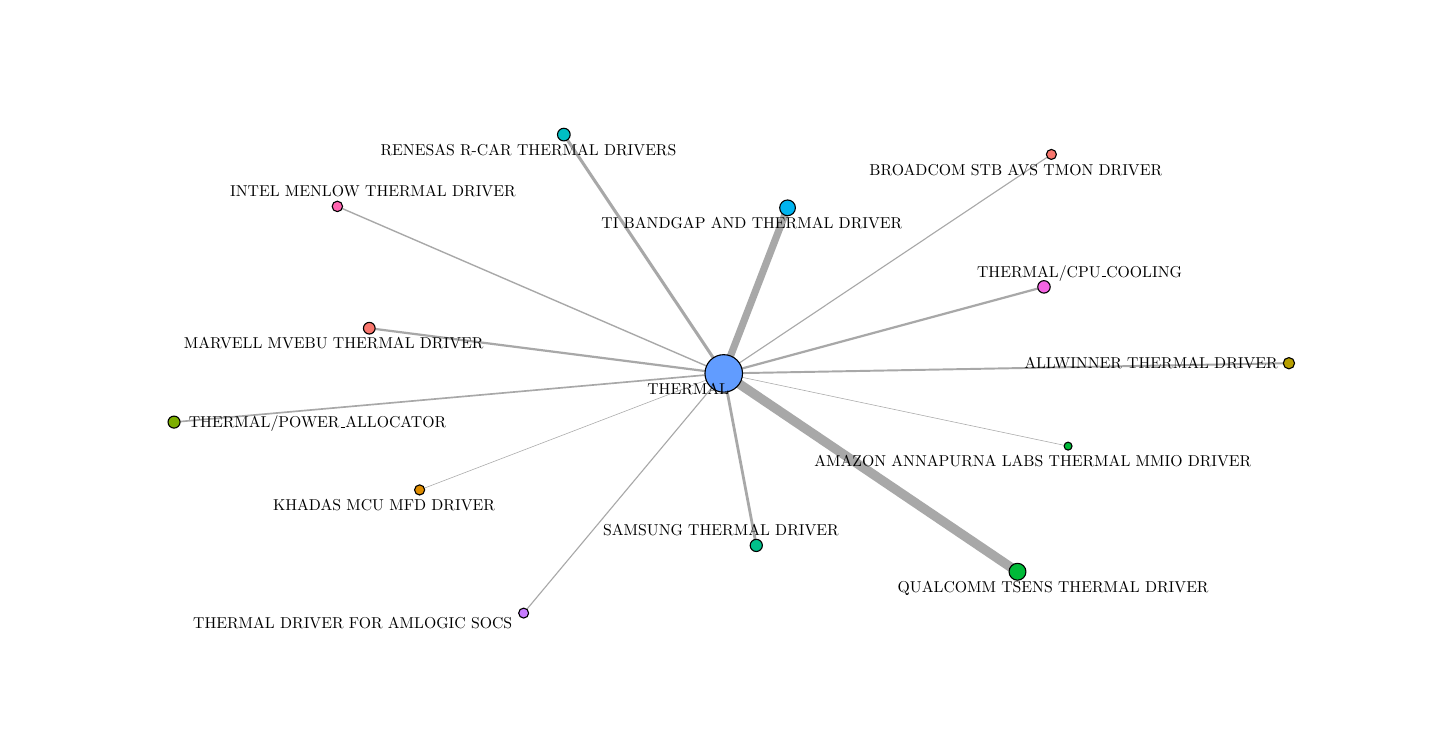
\begin{tikzpicture}[x=1pt,y=1pt]
\definecolor{fillColor}{RGB}{255,255,255}
\path[use as bounding box,fill=fillColor,fill opacity=0.00] (0,0) rectangle (505.89,252.94);
\begin{scope}
\path[clip] (  0.00,  0.00) rectangle (505.89,252.94);
\definecolor{fillColor}{RGB}{255,255,255}

\path[fill=fillColor] (  0.00,  0.00) rectangle (505.89,252.94);
\end{scope}
\begin{scope}
\path[clip] ( 32.75, 32.75) rectangle (475.89,222.94);
\definecolor{drawColor}{gray}{0.66}

\path[draw=drawColor,line width= 0.7pt,line join=round] (455.75,131.69) -- (251.52,128.00);

\path[draw=drawColor,line width= 0.2pt,line join=round] (375.95,101.73) -- (251.52,128.00);

\path[draw=drawColor,line width= 0.4pt,line join=round] (369.92,207.13) -- (251.52,128.00);

\path[draw=drawColor,line width= 0.5pt,line join=round] (111.90,188.35) -- (251.52,128.00);

\path[draw=drawColor,line width= 0.2pt,line join=round] (141.63, 85.90) -- (251.52,128.00);

\path[draw=drawColor,line width= 0.8pt,line join=round] (123.44,144.34) -- (251.52,128.00);

\path[draw=drawColor,line width= 3.4pt,line join=round] (357.67, 56.33) -- (251.52,128.00);

\path[draw=drawColor,line width= 1.1pt,line join=round] (193.74,214.30) -- (251.52,128.00);

\path[draw=drawColor,line width= 1.0pt,line join=round] (263.28, 65.85) -- (251.52,128.00);

\path[draw=drawColor,line width= 0.4pt,line join=round] (251.52,128.00) -- (179.22, 41.40);

\path[draw=drawColor,line width= 0.8pt,line join=round] (251.52,128.00) -- (367.24,159.27);

\path[draw=drawColor,line width= 0.6pt,line join=round] (251.52,128.00) -- ( 52.89,110.41);

\path[draw=drawColor,line width= 2.6pt,line join=round] (251.52,128.00) -- (274.58,187.84);
\definecolor{drawColor}{RGB}{0,0,0}
\definecolor{fillColor}{RGB}{183,159,0}

\path[draw=drawColor,line width= 0.4pt,line join=round,line cap=round,fill=fillColor] (455.75,131.69) circle (  2.04);
\definecolor{fillColor}{RGB}{0,186,56}

\path[draw=drawColor,line width= 0.4pt,line join=round,line cap=round,fill=fillColor] (375.95,101.73) circle (  1.43);
\definecolor{fillColor}{RGB}{248,118,109}

\path[draw=drawColor,line width= 0.4pt,line join=round,line cap=round,fill=fillColor] (369.92,207.13) circle (  1.81);
\definecolor{fillColor}{RGB}{255,100,176}

\path[draw=drawColor,line width= 0.4pt,line join=round,line cap=round,fill=fillColor] (111.90,188.35) circle (  1.89);
\definecolor{fillColor}{RGB}{222,140,0}

\path[draw=drawColor,line width= 0.4pt,line join=round,line cap=round,fill=fillColor] (141.63, 85.90) circle (  1.83);
\definecolor{fillColor}{RGB}{248,118,109}

\path[draw=drawColor,line width= 0.4pt,line join=round,line cap=round,fill=fillColor] (123.44,144.34) circle (  2.11);
\definecolor{fillColor}{RGB}{0,186,56}

\path[draw=drawColor,line width= 0.4pt,line join=round,line cap=round,fill=fillColor] (357.67, 56.33) circle (  3.05);
\definecolor{fillColor}{RGB}{0,191,196}

\path[draw=drawColor,line width= 0.4pt,line join=round,line cap=round,fill=fillColor] (193.74,214.30) circle (  2.29);
\definecolor{fillColor}{RGB}{0,192,139}

\path[draw=drawColor,line width= 0.4pt,line join=round,line cap=round,fill=fillColor] (263.28, 65.85) circle (  2.20);
\definecolor{fillColor}{RGB}{97,156,255}

\path[draw=drawColor,line width= 0.4pt,line join=round,line cap=round,fill=fillColor] (251.52,128.00) circle (  6.78);
\definecolor{fillColor}{RGB}{199,124,255}

\path[draw=drawColor,line width= 0.4pt,line join=round,line cap=round,fill=fillColor] (179.22, 41.40) circle (  1.80);
\definecolor{fillColor}{RGB}{245,100,227}

\path[draw=drawColor,line width= 0.4pt,line join=round,line cap=round,fill=fillColor] (367.24,159.27) circle (  2.25);
\definecolor{fillColor}{RGB}{124,174,0}

\path[draw=drawColor,line width= 0.4pt,line join=round,line cap=round,fill=fillColor] ( 52.89,110.41) circle (  2.17);
\definecolor{fillColor}{RGB}{0,180,240}

\path[draw=drawColor,line width= 0.4pt,line join=round,line cap=round,fill=fillColor] (274.58,187.84) circle (  2.84);

\node[text=drawColor,anchor=base,inner sep=0pt, outer sep=0pt, scale=  0.57] at (405.92,129.73) {ALLWINNER THERMAL DRIVER};

\node[text=drawColor,anchor=base,inner sep=0pt, outer sep=0pt, scale=  0.57] at (363.20, 94.27) {AMAZON ANNAPURNA LABS THERMAL MMIO DRIVER};

\node[text=drawColor,anchor=base,inner sep=0pt, outer sep=0pt, scale=  0.57] at (357.06,199.66) {BROADCOM STB AVS TMON DRIVER};

\node[text=drawColor,anchor=base,inner sep=0pt, outer sep=0pt, scale=  0.57] at (124.75,191.90) {INTEL MENLOW THERMAL DRIVER};

\node[text=drawColor,anchor=base,inner sep=0pt, outer sep=0pt, scale=  0.57] at (128.75, 78.39) {KHADAS MCU MFD DRIVER};

\node[text=drawColor,anchor=base,inner sep=0pt, outer sep=0pt, scale=  0.57] at (110.58,136.84) {MARVELL MVEBU THERMAL DRIVER};

\node[text=drawColor,anchor=base,inner sep=0pt, outer sep=0pt, scale=  0.57] at (370.56, 48.84) {QUALCOMM TSENS THERMAL DRIVER};

\node[text=drawColor,anchor=base,inner sep=0pt, outer sep=0pt, scale=  0.57] at (180.97,206.85) {RENESAS R-CAR THERMAL DRIVERS};

\node[text=drawColor,anchor=base,inner sep=0pt, outer sep=0pt, scale=  0.57] at (250.51, 69.38) {SAMSUNG THERMAL DRIVER};

\node[text=drawColor,anchor=base,inner sep=0pt, outer sep=0pt, scale=  0.57] at (238.67,120.51) {THERMAL};

\node[text=drawColor,anchor=base,inner sep=0pt, outer sep=0pt, scale=  0.57] at (117.44, 35.76) {THERMAL DRIVER FOR AMLOGIC SOCS};

\node[text=drawColor,anchor=base,inner sep=0pt, outer sep=0pt, scale=  0.57] at (380.09,162.82) {THERMAL/CPU{\_{}}COOLING};

\node[text=drawColor,anchor=base,inner sep=0pt, outer sep=0pt, scale=  0.57] at (104.75,108.45) {THERMAL/POWER{\_{}}ALLOCATOR};

\node[text=drawColor,anchor=base,inner sep=0pt, outer sep=0pt, scale=  0.57] at (261.67,180.33) {TI BANDGAP AND THERMAL DRIVER};
\end{scope}
\end{tikzpicture}
